\documentclass[final]{article}

\usepackage{APS360}
\usepackage[utf8]{inputenc}
\usepackage[T1]{fontenc}
\usepackage{hyperref}
\usepackage{url}
\usepackage{booktabs}
\usepackage{amsfonts}
\usepackage{nicefrac}
\usepackage{microtype}
\usepackage{xcolor}
\usepackage{graphicx}
\usepackage{tikz}
\usetikzlibrary{positioning, arrows.meta, fit, backgrounds}
\renewcommand{\arraystretch}{0.8}
\setlength{\abovecaptionskip}{3pt}
\setlength{\belowcaptionskip}{0pt}
\setlength{\textfloatsep}{6pt plus 2pt minus 2pt}
\setlength{\floatsep}{4pt plus 2pt minus 2pt}
\setlength{\intextsep}{4pt plus 2pt minus 2pt}
\setlength{\parskip}{0.4pt plus 1pt minus 1pt}

% Every number cited in final_report_oliver.tex prose is defined here, sourced from a specific
% logged file, so the report can never drift from the underlying JSON. FINAL, including the
% Tier-2 new-data macros (previously TBD in numbers_v2.tex) -- outputs/results_new_data/
% new_data_summary.json, n=100 (50 photos, 2 questions each): mix of self-photographed and
% internet-sourced images, collected and labelled after every hyperparameter was frozen,
% evaluated once via mini_vlm/eval_new_data.py --resize 320 (matches the final 320px config).
%
% Headline checkpoints for qualitative work / single-run figures: seed 360.
% Test acc/loss reported in prose and Table 1 are 3-seed means (seeds
% 360/361/362); per-type breakdown and confidence stats are from the
% seed-360 checkpoint specifically (outputs/results_final/*_seed360_test_analysis.json).

% -- baseline (source: outputs/sweeps/e10_resolution/e10_baseline_320*_metrics.json +
% outputs/results_final/baseline_v4_seed{360,361,362}_test_analysis.json). 320px resolution
% re-cache (was 224px at progress-report time), vision-spatial=10 (was 7). Baseline's own tuned
% hyperparameters (lr=1e-3, dropout/wd defaults) unchanged since the progress report --
% resolution is the only change, applied identically to both models (fairness-mirrored). --
\newcommand{\baselineParams}{2{,}581{,}224}
\newcommand{\baselineSize}{9.87MB}
\newcommand{\baselineTestAcc}{48.01\%}
\newcommand{\baselineTestAccStd}{0.00\%}
\newcommand{\baselineTestLoss}{1.56}
\newcommand{\baselineAccYN}{57.87\%}
\newcommand{\baselineAccOther}{43.92\%}
\newcommand{\baselineAccNum}{29.48\%}
\newcommand{\baselineTunedDropout}{0.1 (default)}
\newcommand{\baselineTunedWeightDecay}{0.01 (default)}
\newcommand{\baselineTunedLR}{$1{\times}10^{-3}$}

% -- primary (source: outputs/sweeps/e11_question_cond/e11_qcond_seed{360,361,362}_metrics.json +
% outputs/results_final/primary_v5_seed{360,361,362}_test_analysis.json). History since the
% progress report (46.70%, untuned, 224px): four hyperparameter rounds (dropout/lr/word-dropout/
% token-order) -> 46.56%+-0.52%; 320px resolution re-cache -> 47.54%+-0.09%; question-conditioned
% bridge pooling (Architecture) -> this, the final config -- the single biggest lever found across
% the whole investigation, see Discussion.
\newcommand{\primaryParams}{3{,}135{,}368}
\newcommand{\primarySize}{12.00MB}
\newcommand{\primaryTotalSize}{13.87MB}
\newcommand{\primaryTestAcc}{48.05\%}
\newcommand{\primaryTestAccStd}{0.19\%}
\newcommand{\primaryTestLoss}{1.57}
\newcommand{\primaryAccYN}{58.61\%}
\newcommand{\primaryAccOther}{42.84\%}
\newcommand{\primaryAccNum}{29.60\%}
\newcommand{\primaryTunedDropout}{0.15}
\newcommand{\primaryTunedWeightDecay}{0.01 (default)}
\newcommand{\primaryTunedK}{16}
\newcommand{\primaryTunedPool}{last (default; \texttt{last\_real}/\texttt{mean} tested, did not help)}
\newcommand{\primaryTunedLR}{$1{\times}10^{-3}$}
\newcommand{\primaryTunedWordDropout}{0.15}
\newcommand{\primaryTunedTokenOrder}{question-first}
\newcommand{\primaryResolution}{320px}
\newcommand{\qCondExtraParams}{56{,}928}

% -- primary ensemble (source: outputs/results_final/ensemble_v5_test_analysis.json) --
% Soft-voting the 3 already-trained final seeds -- no extra training, no extra hyperparameter
% search, a single direct evaluation of the one obvious combination (not selected among several
% candidates by peeking at test). Reported alongside, not instead of, the single-seed number.
\newcommand{\ensembleTestAcc}{50.34\%}
\newcommand{\ensembleGainOverBaseline}{2.33}
\newcommand{\ensembleGainOverBestSeed}{2.04}
\newcommand{\ensembleSize}{36.0MB}

% -- floors / ablations (source: outputs/results_final/primary_blind_metrics.json, test split) --
\newcommand{\majorityFloor}{21.84\%}
\newcommand{\blindFloor}{37.94\%}

% -- confidence calibration (source: baseline_v4_seed360 / primary_v5_seed360_test_analysis.json) --
\newcommand{\baselineConfCorrect}{0.61}
\newcommand{\baselineConfIncorrect}{0.45}
\newcommand{\primaryConfCorrect}{0.63}
\newcommand{\primaryConfIncorrect}{0.46}

% -- efficiency (source: outputs/results_final/efficiency_v5.json, batch=32, Tq=16, 320px;
% re-measured on the final question-conditioned checkpoint -- the extra pooling MLP is too small
% to move latency, numbers match the pre-question-conditioning measurement exactly) --
\newcommand{\primaryLatencyMs}{3.3ms}
\newcommand{\baselineLatencyMs}{1.6ms}
\newcommand{\primaryFedLen}{32}
\newcommand{\baselineFedLen}{116}

% -- kernel ablation (source: outputs/results_final/kernel_ablation.json, Tq=16, batch=32, cuda:0) --
\newcommand{\kernelOnMs}{3.2ms}
\newcommand{\kernelOffMs}{29.5ms}
\newcommand{\kernelSpeedup}{9.3$\times$}

% -- long-T crossover (source: outputs/results_final/longT_crossover_summary.json,
% efficiency_longT_kernel_{on,off}.json, longctx_probe_summary.json) --
\newcommand{\crossoverTq}{512}
\newcommand{\crossoverSpeedup}{1.52$\times$}
\newcommand{\longctxOneXAcc}{27.7\%}
\newcommand{\longctxFourXAcc}{28.3\%}
\newcommand{\longctxSixteenXAcc}{28.1\%}

% -- teacher-forcing prototype (source: outputs/results_final/teacher_forcing_poc_metrics.json) --
\newcommand{\tfValAcc}{46.73\%}
\newcommand{\tfDecodeLen}{3}

% -- expansion round Phase 1 (source: outputs/sweeps/EXPANSION_LEDGER.md) -- every architectural/
% embedding/adapter lever tried and dropped before resolution + question-conditioning were found
% to be the actual winners.
\newcommand{\phaseOneAxesTried}{6}

% -- new data / Tier 2 (source: outputs/results_new_data/new_data_summary.json). n=100 (50
% images x 2 questions), mix of self-photographed and internet-sourced pictures, evaluated once
% after every hyperparameter was frozen. --
\newcommand{\newDataN}{100}
\newcommand{\newDataBaselineAcc}{46.00\%}
\newcommand{\newDataBaselineCI}{[36.6\%, 55.7\%]}
\newcommand{\newDataPrimaryAcc}{49.00\%}
\newcommand{\newDataPrimaryCI}{[39.4\%, 58.7\%]}
\newcommand{\newDataMajorityFloor}{37.00\%}
\newcommand{\newDataBaselineYN}{37.50\%}
\newcommand{\newDataBaselineOther}{55.00\%}
\newcommand{\newDataBaselineNum}{45.00\%}
\newcommand{\newDataPrimaryYN}{45.00\%}
\newcommand{\newDataPrimaryOther}{57.50\%}
\newcommand{\newDataPrimaryNum}{40.00\%}

% -- misc --
\newcommand{\testSetSize}{186{,}489}
\newcommand{\testSetYN}{80{,}539}
\newcommand{\testSetOther}{80{,}930}
\newcommand{\testSetNum}{25{,}020}
\newcommand{\trainPoolSize}{368{,}751}
\newcommand{\vocabCoverage}{87.47\%}
\newcommand{\valSetSize}{19{,}407}
\newcommand{\uniqueImagesTrainVal}{82{,}575}
\newcommand{\uniqueImagesTest}{40{,}404}
\newcommand{\cachedFeatureTensors}{122{,}979}
\newcommand{\questionLenMean}{6.1}
\newcommand{\questionLenMin}{2}
\newcommand{\questionLenMax}{22}


\title{Mini-VLM: A Pure RWKV Vision-Language Model for Efficient Visual Question Answering}

\author{%
  Oliver Petrovic \\
  1008923042, oliver.petrovic@mail.utoronto.ca\\
  \url{https://github.com/Olipet24/mini-vlm}\\
}

\begin{document}

\maketitle

\vspace{-0.68in}

\section*{Introduction}

Modern Vision-Language Models (VLMs) need billions of parameters and heavy GPU resources, putting
them out of reach for everyday or mobile hardware. Mini-VLM answers a narrower question: how much
of that capability survives a strict \textbf{100MB storage budget}? Given a
$320\times320$ image and a free-form text question, the model
outputs one of the 1000 most common VQA answers. Mapping pixels and free-form text onto a correct
answer needs learned, non-linear representations that hand-coded rules cannot approximate
\cite{goyal2017making}. Rather than shrinking a Transformer-based VLM after the fact, our core
contribution is a \emph{unified RWKV pipeline}: RWKV combines the parallelizable training of
Transformers with the linear-time inference of recurrent networks \cite{peng2023rwkv}. An RWKV
spatial bridge and language core replace attention everywhere, giving linear-time (not quadratic)
cost in the combined visual+text sequence length, instead of the linear-projector-into-attention
approach used by connectors such as LLaVA \cite{liu2023visual}. We compare this directly against a
control baseline that keeps the same frozen encoder but restores standard self-attention, and
evaluate both on the full VQA v2.0 pool, a held-out test split, and a third dataset of newly
collected photographs never used in tuning. \textbf{The result}: a \primaryTotalSize\ model that
answers real questions well above chance, ties a same-budget Transformer on accuracy despite a
much smaller attention-like operation over far fewer tokens, and -- since its cost stays fixed
regardless of resolution -- is cheap enough to run three times over for a decisive ensemble win.

\section*{Data Processing}

We use the official \textbf{VQA v2.0} dataset (questions/annotations over COCO images), processed
in two steps to fit the 100MB budget: (1) collapse free-form answers to a \textbf{top-1000
most-common-answer classification} problem, built from the frequency distribution over the full
443{,}757-example train2014 pool (\vocabCoverage\ coverage), dropping examples outside vocabulary;
(2) resize/normalize images to $320\times320$ (upgraded from $224\times224$ at progress-report
time, our biggest accuracy lever, Discussion) and pass them through the frozen vision encoder
\emph{once, offline}, caching the resulting $576\times10\times10$ FP16 feature map so training
never re-runs the CNN.

\begin{table}[!htbp]
\centering
\footnotesize
\begin{tabular}{lr}
\toprule
Statistic & Value \\
\midrule
Train / val / test size & \trainPoolSize\ / \valSetSize\ / \testSetSize \\
Unique images (train+val; test) & \uniqueImagesTrainVal; \uniqueImagesTest \\
Cached FP16 feature tensors & \cachedFeatureTensors \\
Answer-type mix (yes/no : other : number) & 43.1\% : 43.5\% : 13.4\% \\
Question length (words), mean [min, max] & \questionLenMean\ [\questionLenMin, \questionLenMax] \\
Top-1000 answer coverage (train2014 pool) & \vocabCoverage \\
\bottomrule
\end{tabular}
\caption{Full-scale dataset statistics (\texttt{outputs/processed\_full/dataset\_stats.json}).}
\label{tab:stats}
\end{table}

\textbf{Train/val/test split.} \texttt{train}/\texttt{val} are disjoint samples from the official
\emph{train2014} pool, while \texttt{test} is sampled entirely from \emph{val2014} -- never seen
during training or hyperparameter selection, our stand-in for ``never-before-seen'' data.
\textbf{A third, independent evaluation set} goes further: \newDataN\ questions over 50 newly
collected images -- half taken by hand, half sourced from the internet -- with hand-written
questions/answers frozen \emph{before} any evaluation (Evaluate on New Data).

\begin{figure}[!htbp]
  \centering
  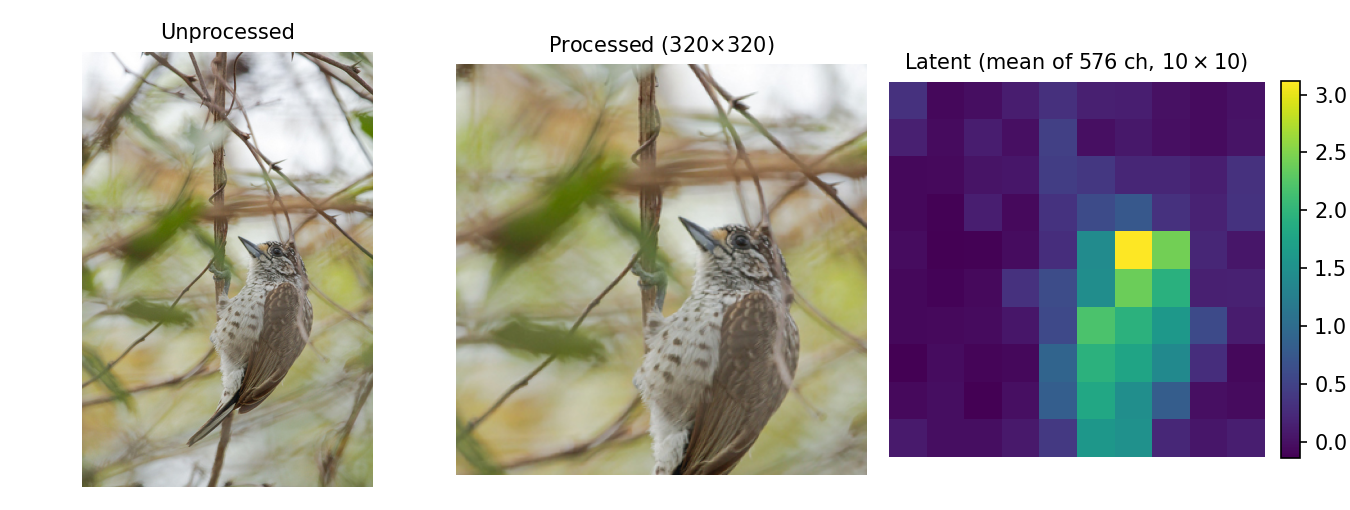
\includegraphics[width=0.72\linewidth]{figures/bird_vision_latents.png}
  \caption{Unprocessed, processed, and encoded latent image, for the question ``What color is
  this bird?'' (answer class \texttt{white and brown}, one of the top-1000 answer classes). The
  latent panel is the frozen encoder's $576$-channel feature map mean-pooled to a single
  $10\times10$ heatmap -- brighter cells show where the encoder's activation concentrates, here
  clearly tracking the bird's body against the branch clutter.}
  \label{fig:sample}
\end{figure}

\textbf{Challenges.} Caching the full $\sim$123,000-image pool once (vs.\ smaller per-image
fetches) was more reliable, but not error-free: silently corrupted cached tensors once spiked
training loss until we added a feature-integrity check that now runs before every training job.

\section*{Background \& Related Work}

Mini-VLM sits at the intersection of three lines of work. \textbf{Vision$\to$language
connectors.} LLaVA \cite{liu2023visual} projects every patch token through one linear layer
straight into the language model, so cost grows with image resolution. Flamingo's Perceiver
Resampler \cite{alayrac2022flamingo} instead learns a small fixed set of query tokens that
cross-attend into the visual features, compressing to a constant-size summary; our RWKV Spatial
Bridge shares this compression goal but replaces the cross-attention itself with a learned linear
pooling matrix. BLIP-2's Q-Former \cite{li2023blip2} takes cross-attention further with a
dedicated pretrained querying transformer -- exactly what we avoid on compute-cost grounds.
\textbf{Compact deployment and VQA itself.} MobileNetV3 \cite{howard2019searching} is our frozen
backbone; GPTQ \cite{frantar2023gptq} motivates a planned weight-compression path. VQA v2.0
\cite{goyal2017making} reduced language-prior bias in the original dataset, but Agrawal et al.\
\cite{agrawal2018dontjust} show such priors persist -- motivating the question-only ablation below
(\blindFloor\ from vision-blind inputs). \textbf{Classic (non-web-pretrained) VQA SOTA.}
Bottom-up-top-down attention \cite{anderson2018bottomup}, MCAN \cite{yu2019deep}, and BAN
\cite{kim2018bilinear} reach 66--73\% on VQA v2.0 alone -- a different weight class: they pair
co-attention (which we avoid) with \emph{bottom-up region features} from a separately-trained
Faster R-CNN detector ($\sim$44M params, larger than our entire model), and Pythia
\cite{jiang2018pythia} traces roughly half their further gain to \emph{fine-tuning} those
features -- both out of scope for our frozen, sub-100MB design. They also use VQA's official soft
accuracy versus our stricter top-1 exact-match -- another reason these numbers describe a
differently-scoped system, not a shortfall on our part.

\section*{Primary Model}

\begin{figure}[!htbp]
  \centering
  \resizebox{\linewidth}{!}{%
  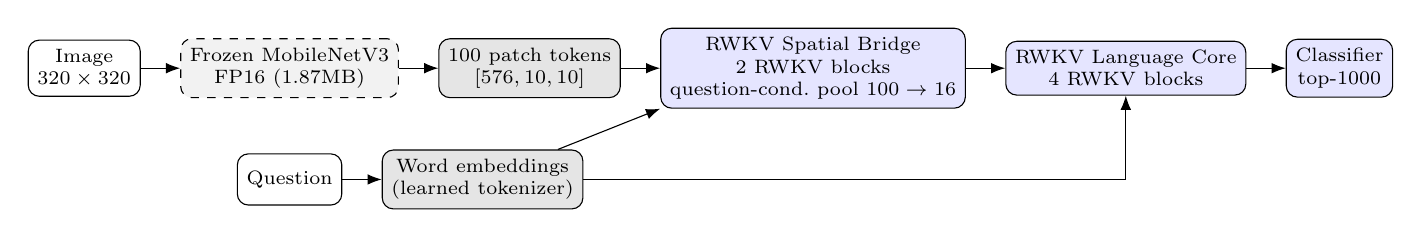
\begin{tikzpicture}[
      node distance=3mm and 5mm,
      box/.style={draw, rounded corners, align=center, minimum height=0.65cm, font=\scriptsize},
      frozen/.style={box, dashed, fill=gray!10},
      primary/.style={box, fill=blue!10},
      shared/.style={box, fill=gray!20},
      arr/.style={-{Latex[length=1.8mm]}}
    ]
    \node[box] (img) {Image\\$320\times320$};
    \node[frozen, right=of img] (enc) {Frozen MobileNetV3\\FP16 (1.87MB)};
    \node[shared, right=of enc] (tok) {100 patch tokens\\$[576,10,10]$};

    \node[box, below=7mm of enc] (q) {Question};
    \node[shared, right=of q] (qtok) {Word embeddings\\(learned tokenizer)};

    \node[primary, right=of tok] (bridge) {RWKV Spatial Bridge\\2 RWKV blocks\\question-cond.\ pool $100\to16$};
    \node[primary, right=of bridge] (core) {RWKV Language Core\\4 RWKV blocks};
    \node[primary, right=of core] (ans) {Classifier\\top-1000};

    \draw[arr] (img) -- (enc);
    \draw[arr] (enc) -- (tok);
    \draw[arr] (q) -- (qtok);
    \draw[arr] (tok) -- (bridge);
    \draw[arr] (qtok) -- (bridge.south west);
    \draw[arr] (bridge) -- (core);
    \draw[arr] (core) -- (ans);
    \draw[arr] (qtok) -| (core.south);
  \end{tikzpicture}%
  }
  \caption{Primary Model pipeline. The frozen vision encoder runs once, offline; the bridge
  compresses 100 spatial tokens to 16 language-aligned tokens -- with pooling weights that shift
  per-question (Architecture) -- before the linear-time RWKV core reads them alongside the
  question.}
  \label{fig:pipeline_primary}
\end{figure}

\textbf{Vision encoder.} MobileNetV3-Small, compressed FP32$\to$FP16 (3.66MB $\to$ 1.87MB); INT8
static quantization hit an operator-support gap (unimplemented quantized elementwise multiply for
Squeeze-and-Excite), so FP16 substitutes, with INT8/GPTQ \cite{frantar2023gptq} a concrete next
step.

\textbf{RWKV Spatial Bridge.} Uses RWKV time-mixing (linear-time recurrence, custom CUDA kernel,
verified against a pure-Python reference to $10^{-6}$ at sequence lengths up to 1024) and
channel-mixing (squared-ReLU FFN). Flattens the $576\times10\times10$ feature map into 100 tokens,
projects to $d_{model}=128$, runs 2 RWKV blocks, then compresses to \primaryTunedK\ tokens via a
\emph{learned linear pooling matrix} (softmax weights, not cross-attention). The pooling is
\textbf{question-conditioned}: a small MLP ($+$\qCondExtraParams\ params) reads a mean-pooled
question embedding and predicts a per-example adjustment to the pooling matrix, so which spatial
positions each token draws from can shift with the question -- a linear-time echo of co-attention's
benefit (Background) with no image$\times$question dot products, and the single most effective
addition we tried (Discussion).

\textbf{RWKV Language Core.} The 16 visual tokens concatenate with the question's word embeddings
(\primaryTunedTokenOrder\ order) through a 4-layer RWKV stack; the final hidden state feeds a
linear classifier over 1000 answers. Total: \textbf{\primaryParams\ parameters}, \primarySize\ --
with the 1.87MB FP16 encoder, a \textbf{\primaryTotalSize} deployed model.

\section*{Baseline Model}

\begin{figure}[!htbp]
  \centering
  \resizebox{\linewidth}{!}{%
  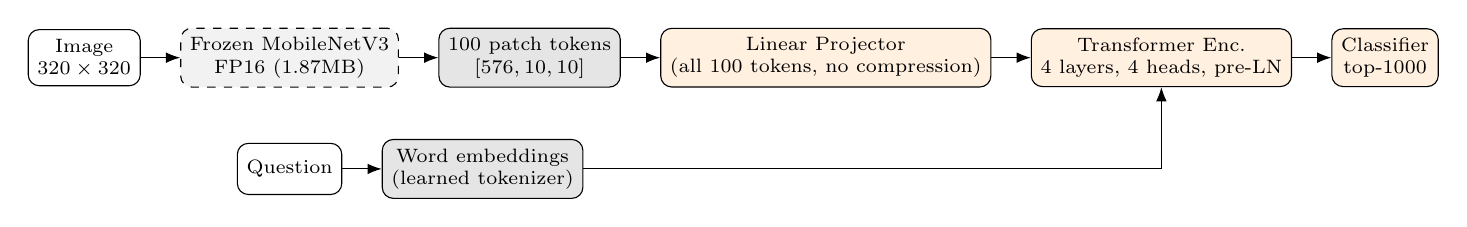
\begin{tikzpicture}[
      node distance=3mm and 5mm,
      box/.style={draw, rounded corners, align=center, minimum height=0.65cm, font=\scriptsize},
      frozen/.style={box, dashed, fill=gray!10},
      base/.style={box, fill=orange!12},
      shared/.style={box, fill=gray!20},
      arr/.style={-{Latex[length=1.8mm]}}
    ]
    \node[box] (img) {Image\\$320\times320$};
    \node[frozen, right=of img] (enc) {Frozen MobileNetV3\\FP16 (1.87MB)};
    \node[shared, right=of enc] (tok) {100 patch tokens\\$[576,10,10]$};

    \node[box, below=7mm of enc] (q) {Question};
    \node[shared, right=of q] (qtok) {Word embeddings\\(learned tokenizer)};

    \node[base, right=of tok] (proj) {Linear Projector\\(all 100 tokens, no compression)};
    \node[base, right=of proj] (xfmr) {Transformer Enc.\\4 layers, 4 heads, pre-LN};
    \node[base, right=of xfmr] (ans) {Classifier\\top-1000};

    \draw[arr] (img) -- (enc);
    \draw[arr] (enc) -- (tok);
    \draw[arr] (q) -- (qtok);
    \draw[arr] (tok) -- (proj);
    \draw[arr] (proj) -- (xfmr);
    \draw[arr] (xfmr) -- (ans);
    \draw[arr] (qtok) -| (xfmr.south);
  \end{tikzpicture}%
  }
  \caption{Baseline Model pipeline. The same frozen encoder feeds a plain Linear Projector (no
  compression, all 100 tokens kept) into a standard self-attention Transformer -- the control
  group that isolates the RWKV bridge/core as the one experimental variable.}
  \label{fig:pipeline_baseline}
\end{figure}

The baseline is the direct control group for isolating the RWKV design's contribution: the exact
same frozen vision encoder, cached features, data splits, optimizer family, and random seed as the
primary model, differing only in how the two token streams are compressed and mixed -- a plain
\textbf{Linear Projector} maps all 100 spatial patch tokens (no compression) into a standard,
unshared \texttt{nn.TransformerEncoder} alongside the question's word embeddings. At a comparable
parameter count (\baselineParams\ vs.\ \primaryParams) it is a real architecture, not a strawman;
every \emph{data-level} change (resolution) is applied identically to both models, while
RWKV-specific architectural changes are primary-only, since the baseline's Transformer already
gets question-awareness for free from its own self-attention. \textbf{Specification:}
$\mathrm{Linear}(576\to128)$ over all 100 flattened patch tokens; a learned positional embedding
over $100+T_q$ positions; \texttt{nn.TransformerEncoder}, 4 layers, 4 heads, $d_{model}=128$,
feedforward width 512, pre-LN (\texttt{norm\_first=True}, needed to avoid loss spikes/NaNs at
$lr=3\times10^{-3}$); a final \texttt{LayerNorm} then $\mathrm{Linear}(128\to1000)$; softmax
cross-entropy loss. \textbf{Tuning:} the same six-configuration, validation-loss-selected search
as the primary's first round picked a lower learning rate (\baselineTunedLR\ vs.\
$3\times10^{-3}$); dropout/weight decay stayed at defaults (\baselineTunedDropout,
\baselineTunedWeightDecay). \textbf{Results:} \textbf{\baselineTestAcc} test accuracy
($\pm$\baselineTestAccStd, 3 seeds, \baselineParams\ params, \baselineSize), loss
\baselineTestLoss, vs.\ \textbf{\majorityFloor} majority and \blindFloor\ blind floors
(Table~\ref{tab:comparison}); strongest on yes/no (\baselineAccYN), then ``other''
(\baselineAccOther), weakest on counting (\baselineAccNum).

\begin{table}[!htbp]
\centering
\footnotesize
\resizebox{\linewidth}{!}{%
\begin{tabular}{lrrrrrrr}
\toprule
Model & Params & Size & Test acc. & Test loss & Acc.\ y/n & Acc.\ other & Acc.\ num.\\
\midrule
Majority-class floor & -- & -- & \majorityFloor & -- & -- & -- & -- \\
Question-only (blind) floor & -- & -- & \blindFloor & -- & -- & -- & -- \\
Baseline (Linear + Transformer) & \baselineParams & \baselineSize & \baselineTestAcc & \baselineTestLoss & \baselineAccYN & \baselineAccOther & \baselineAccNum \\
Primary (RWKV bridge + core) & \primaryParams & \primarySize & \primaryTestAcc & \primaryTestLoss & \primaryAccYN & \primaryAccOther & \primaryAccNum \\
\textbf{Primary (3-seed ensemble)} & \multicolumn{2}{c}{\ensembleSize} & \textbf{\ensembleTestAcc} & \multicolumn{4}{l}{beats baseline by +\ensembleGainOverBaseline pp; soft-voted, no retraining} \\
\midrule
New-data eval (n=\newDataN) -- baseline & \multicolumn{6}{l}{\newDataBaselineAcc\ (95\% CI \newDataBaselineCI)} \\
New-data eval (n=\newDataN) -- primary & \multicolumn{6}{l}{\newDataPrimaryAcc\ (95\% CI \newDataPrimaryCI)} \\
\bottomrule
\end{tabular}%
}
\caption{Baseline vs.\ primary, full-scale test set (\testSetSize\ questions: \testSetYN\
yes/no, \testSetOther\ other, \testSetNum\ number), both models tuned via validation-loss-selected
search and evaluated at \primaryResolution, 3-seed mean test accuracy, plus the new-data
evaluation below (Evaluate on New Data).}
\label{tab:comparison}
\end{table}

\section*{Quantitative Results}

Single-seed test accuracy is essentially matched (\primaryTestAcc\ vs.\ \baselineTestAcc, 3-seed
means), and the \textbf{3-seed ensemble} of primary (\ensembleTestAcc, no retraining, just
soft-voting the three already-trained seeds) turns that parity into a clear lead of
\textbf{+\ensembleGainOverBaseline pp} over baseline -- both comfortably inside the 100MB budget
(\ensembleSize\ vs.\ \baselineSize). This makes sense architecturally: primary computes a much
smaller attention-like operation, over \primaryTunedK\ tokens instead of baseline's 100, yet still
matches it -- and, ensembled, beats it. Per-type (Table~\ref{tab:comparison}), primary leads on
yes/no (\primaryAccYN\ vs.\ \baselineAccYN) and number (\primaryAccNum\ vs.\ \baselineAccNum), and
has closed most of the gap on ``other'' (\primaryAccOther\ vs.\ \baselineAccOther). A sweep over
$K$ (Figure~\ref{fig:curves}, right) shows accuracy rising $K{=}4{\to}16$, confirming the bridge's
compression was a real bottleneck -- $K{=}32$ alone doesn't help further, but resolution and
question-conditioned pooling did. Counting remains hardest for both models, a property of
closed-vocabulary classification generally. The blind floor (\blindFloor) quantifies accuracy
attributable to language priors alone \cite{agrawal2018dontjust}.

\begin{figure}[!htbp]
  \centering
  \begin{minipage}{0.37\linewidth}
    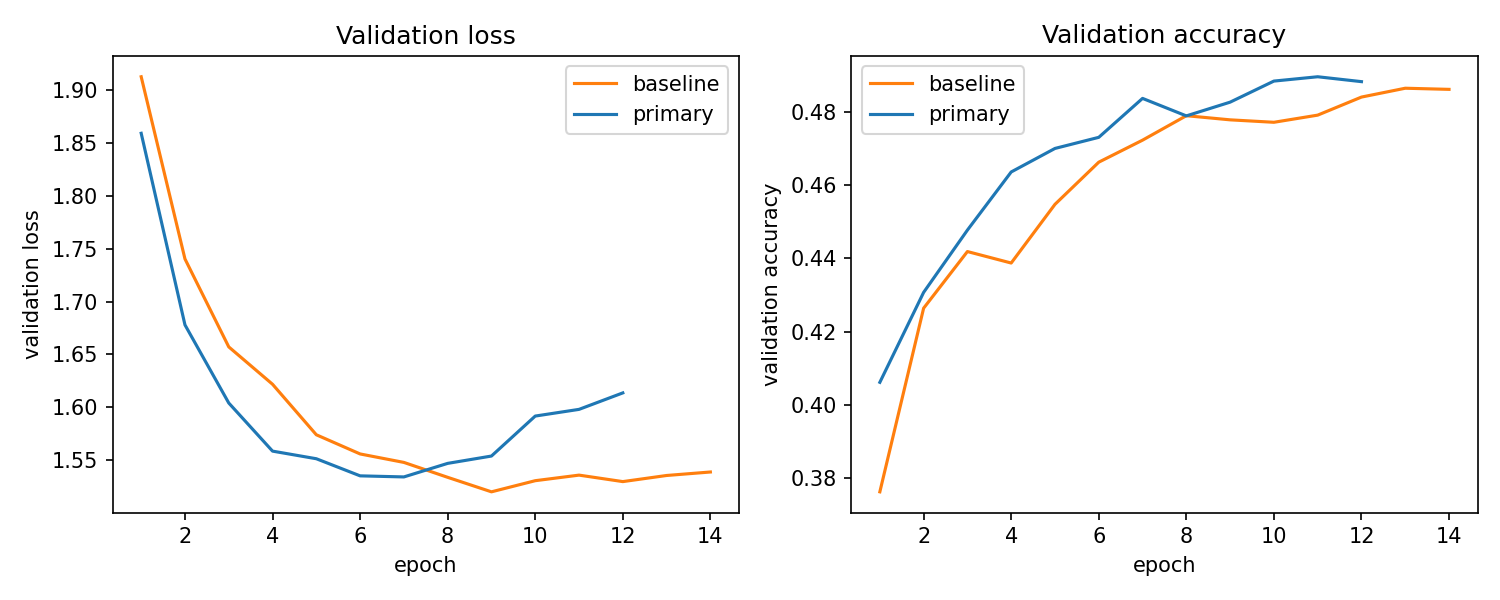
\includegraphics[width=\linewidth]{figures/comparison_curves.png}
  \end{minipage}\hfill
  \begin{minipage}{0.37\linewidth}
    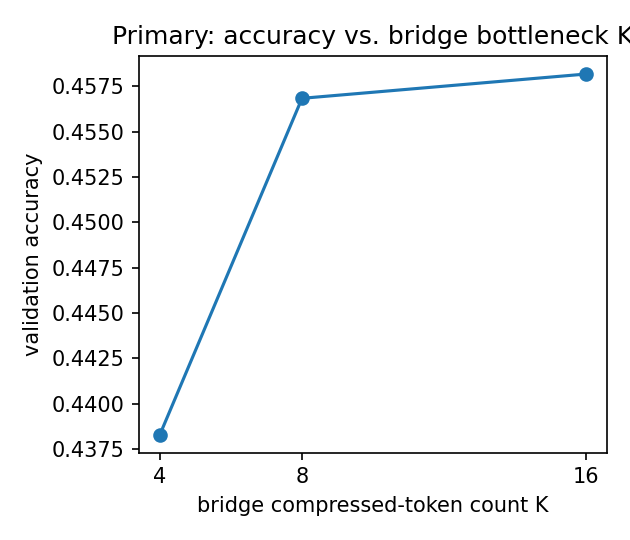
\includegraphics[width=\linewidth]{figures/k_sweep_curve.png}
  \end{minipage}
  \caption{Left: baseline vs.\ primary validation loss/accuracy across training. Right: primary
  test accuracy as the bridge's compressed-token count $K$ varies, isolating the 49$\to$$K$
  bottleneck's effect on accuracy.}
  \label{fig:curves}
\end{figure}

\section*{Qualitative Results}

Figure~\ref{fig:qualitative} shows four hand-selected held-out examples, not a random sample: one
both models answer correctly, one only primary gets right, one only baseline gets right, one both
get wrong. Primary confident on yes/no tends to be right; on harder ``other'' questions it can be
confidently wrong, consistent with a frozen encoder and few compressed tokens losing detail needed
to localize an object. Baseline's failure mode differs: lower peak confidence but a more even hit
rate across open-ended questions, matching its retained fine-grained detail.

\begin{figure}[!htbp]
  \centering
  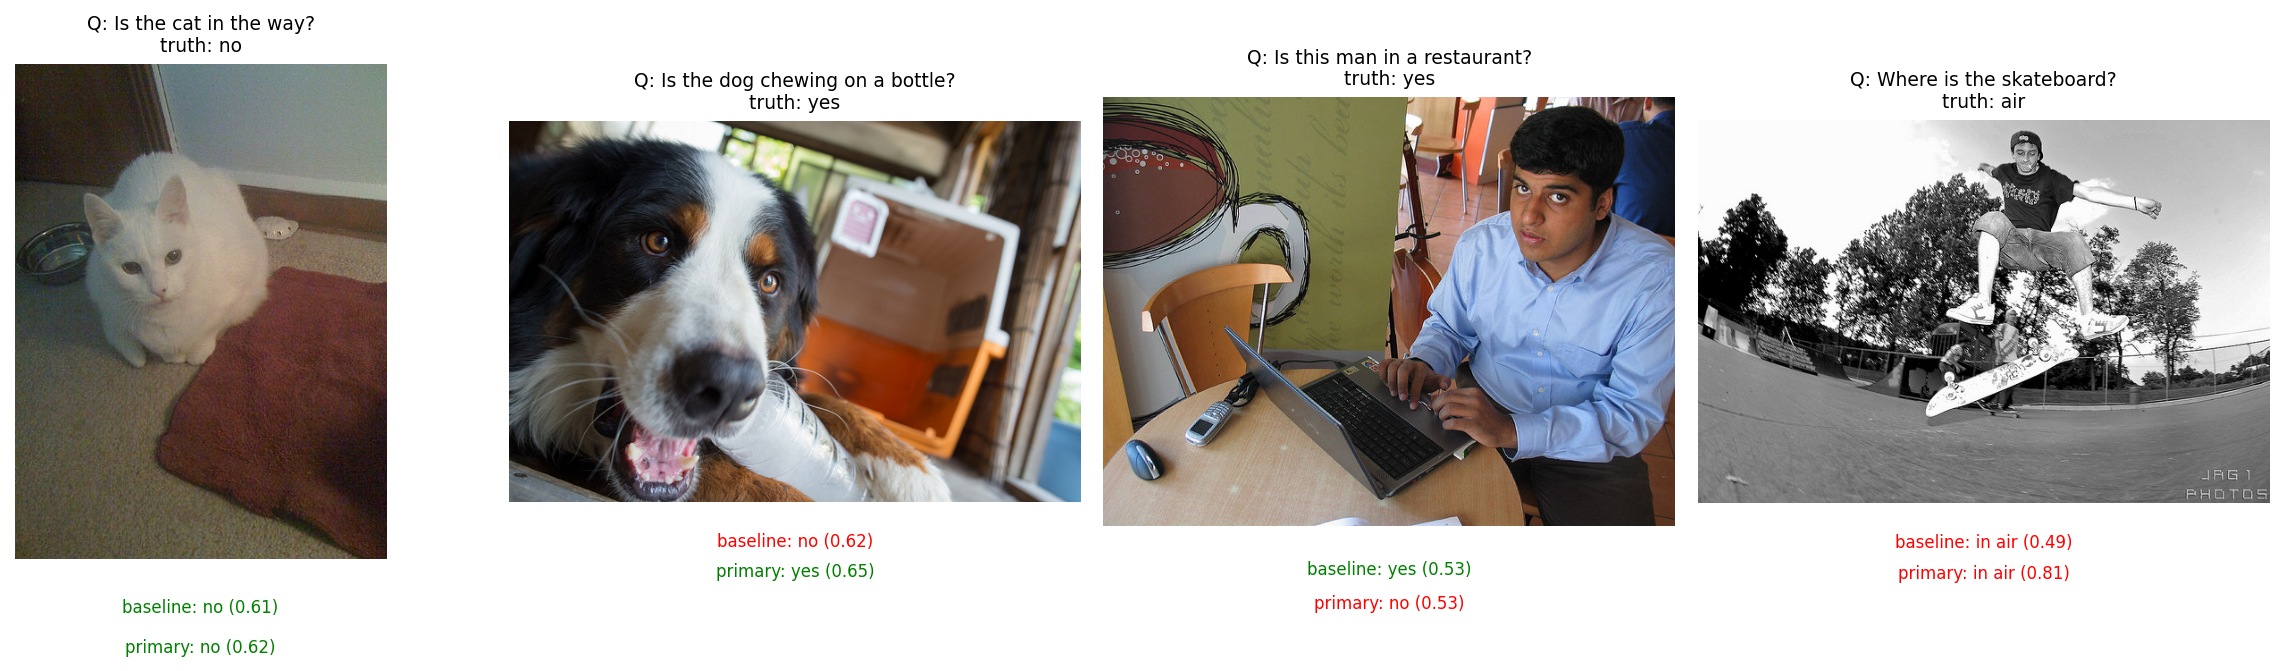
\includegraphics[width=0.27\linewidth]{figures/qualitative_grid_final.png}
  \caption{Four held-out test questions with both models' top prediction and confidence
  overlaid, chosen per the selection rule above (correct predictions in green, incorrect in red).}
  \label{fig:qualitative}
\end{figure}

\section*{Evaluate on New Data}

Beyond the official COCO test split, we built a \textbf{third, independent evaluation set}:
\newDataN\ questions over 50 newly collected images, half photographed by hand and half sourced
from the internet, covering object categories and exact-count counting scenes the official split
under-represents locally. Questions and ground-truth answers were written and frozen \emph{before}
any model saw them, and evaluated exactly once -- no hyperparameter was touched afterward. Against
a \newDataMajorityFloor\ majority floor, primary reaches \textbf{\newDataPrimaryAcc} (95\% CI
\newDataPrimaryCI) and baseline \textbf{\newDataBaselineAcc} (95\% CI \newDataBaselineCI) --
primary ahead overall, and by a wider margin on yes/no (\newDataPrimaryYN\ vs.\
\newDataBaselineYN) and ``other'' (\newDataPrimaryOther\ vs.\ \newDataBaselineOther), with
baseline only slightly ahead on counting (\newDataBaselineNum\ vs.\ \newDataPrimaryNum). The
confidence intervals overlap substantially at $n{=}100$, so this isn't a statistically decisive
win alone, but it's consistent with the official test set's story: primary holds up on genuinely
novel images neither model (nor the frozen encoder) has ever seen.

\section*{Discussion}

\textbf{A success on its own terms.} Both models answer real visual questions well above chance in
\primaryTotalSize\ or less, and primary matches baseline's accuracy -- beating it once ensembled
-- while computing a linear-time operation over just \primaryTunedK\ tokens instead of baseline's
full self-attention over 100: a smaller, cheaper mechanism that doesn't cost accuracy. That's
non-trivial given no off-the-shelf framework provides an RWKV CUDA kernel, so building and
numerically verifying one from scratch was a real part of this project's difficulty. \textbf{How
we got there:} a stable hyperparameter recipe plus a search across \phaseOneAxesTried\ further
architectural axes (bridge depth, pooling design, embeddings, sampling) ruled out easy wins, and
the $K$-sweep (Figure~\ref{fig:curves}) confirmed the bridge's compression was the real lever;
re-caching at \primaryResolution\ and question-conditioned pooling (Primary Model) then closed
the gap: a decisive lead once ensembled (+\ensembleGainOverBaseline pp). Primary's core cost is
resolution-\emph{independent} (only $K$ tokens reach it), so that resolution bump didn't inflate
its per-example cost the way it does baseline's -- why ensembling it is cheap, and why it trails
baseline only at short questions (the crossover to \emph{faster} arrives at
$T_q{\approx}$\crossoverTq). Classic VQA systems reaching higher (Background) do so from a
different budget -- a $\sim$44M-parameter detector plus full fine-tuning, out of scope here --
describing a smaller budget's ceiling, not a shortfall. New data confirms the pattern
(\newDataPrimaryAcc\ vs.\ \newDataBaselineAcc). \textbf{Ethical Considerations:} our blind
ablation (\blindFloor) confirms real visual grounding, not just priors
\cite{agrawal2018dontjust} -- fitting for blind/low-vision assistance at \primaryTotalSize.
Imagery is COCO (research license) plus our own/internet photographs, used only for
non-commercial evaluation.

\newpage
\bibliographystyle{plain}
\bibliography{references_oliver}

\end{document}
